% Check-in 1 slides, 6.3930. Nine slides for seven minutes, two backup slides.
% Build: pdflatex check-in-1.tex (twice). Needs beamer, tikz, pgfplots, booktabs.
% Rehearsal view with speaker notes: uncomment the \setbeameroption line below.
\documentclass[aspectratio=169,10pt]{beamer}
\usepackage[T1]{fontenc}
\usepackage[utf8]{inputenc}
\usepackage[sfdefault,lining]{FiraSans} % delete this line if the font is not installed
\usepackage{array}
\usepackage{booktabs}
\usepackage{tikz}
\usepackage{pgfplots}
\pgfplotsset{compat=1.17}
\usetikzlibrary{arrows.meta,positioning}
%\usepackage{pgfpages}\setbeameroption{show notes on second screen=right}

% ---------- colours: one hue per corpus, the same on every slide ----------
\definecolor{ink}{HTML}{0B0B0B}
\definecolor{ink2}{HTML}{52514E}
\definecolor{hair}{HTML}{D9D8D3}
\definecolor{tint}{HTML}{EEF3FA}
\definecolor{accent}{HTML}{104281}
\definecolor{cPub}{HTML}{2A78D6}  % PubChem
\definecolor{cZinc}{HTML}{EB6834} % ZINC sample
\definecolor{cCoco}{HTML}{1BAF7A} % COCONUT
\definecolor{cZnp}{HTML}{EDA100}  % ZINC, most natural-product-like tenth

% ---------- look ----------
\setbeamertemplate{navigation symbols}{}
\setbeamercolor{normal text}{fg=ink,bg=white}
\setbeamercolor{frametitle}{fg=ink,bg=white}
\setbeamerfont{frametitle}{series=\bfseries,size=\Large}
\setbeamersize{text margin left=9mm,text margin right=9mm}
\setbeamertemplate{frametitle}{%
  \vspace{5mm}%
  \parbox[t]{\textwidth}{\raggedright\usebeamerfont{frametitle}%
    \usebeamercolor[fg]{frametitle}\insertframetitle\par}%
  \vspace{1mm}}
\setbeamercolor{itemize item}{fg=accent}
\setbeamertemplate{itemize item}{\rule[0.25ex]{0.45em}{0.45em}}
\newcommand{\footlabel}{\insertframenumber}
\setbeamertemplate{footline}{\hfill{\color{ink2}\scriptsize\footlabel}\hspace{7mm}\vspace{3.5mm}}
\newcommand{\muted}[1]{\textcolor{ink2}{#1}}
\newcommand{\key}[1]{{\bfseries\color{accent}#1}}
\newcommand{\sw}[1]{\textcolor{#1}{\rule[-0.1ex]{0.75em}{0.75em}}\hspace{0.4em}}
\newcolumntype{L}[1]{>{\raggedright\arraybackslash}p{#1}}
\hyphenpenalty=10000 \exhyphenpenalty=10000
\setlength{\tabcolsep}{4pt}

\pgfplotsset{
  clean/.style={
    axis line style={draw=none},
    tick style={draw=none},
    grid style={hair,line width=0.4pt},
    label style={font=\small,color=ink2},
    tick label style={font=\small,color=ink2},
    legend style={draw=none,fill=none,font=\small,text=ink},
    legend cell align=left,
    /pgf/number format/assume math mode=true, % numbers in the text font
  },
  swatch legend/.style={legend image code/.code={%
    \fill[##1] (0cm,-0.11cm) rectangle (0.32cm,0.16cm);}},
}

\begin{document}

% =====================================================================
\begin{frame}[plain]
\vspace{16mm}
{\color{accent}\rule{18mm}{1.2mm}}\par\vspace{5mm}
{\fontsize{25}{31}\selectfont\bfseries Does the pretraining corpus matter\\
for molecular property prediction?\par}
\vspace{6mm}
{\Large\muted{Same model. Same training. Different molecules.}\par}
\vfill
{\large Gabriel Dupuis \qquad L\'eonard Mauvernay\par}
\vspace{1.5mm}
{\muted{6.3930 \;\textbullet\; Check-in 1 \;\textbullet\; November 2026}\par}
\vspace{9mm}
\note{15 s. Say the question once, in the words of the title. Then: ``we change
one thing, the molecules a model studies before it sees any measurement.''}
\end{frame}

% =====================================================================
\begin{frame}{Pretraining transformed language and protein models.\\
For molecules, it barely helps.}
\centering
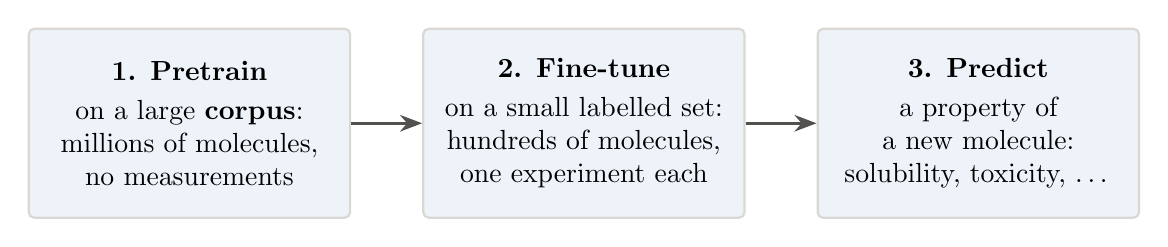
\begin{tikzpicture}[
  node distance=9mm,
  stage/.style={draw=hair,line width=0.8pt,rounded corners=2pt,fill=tint,
    minimum height=24mm,text width=38mm,align=center,inner sep=4pt},
  arr/.style={-{Stealth[length=2.8mm]},line width=1.1pt,color=ink2}]
\node[stage] (a) {\textbf{1. Pretrain}\\[2pt]on a large \textbf{corpus}:\\millions of
  molecules,\\no measurements};
\node[stage,right=of a] (b) {\textbf{2. Fine-tune}\\[2pt]on a small labelled set:\\
  hundreds of molecules,\\one experiment each};
\node[stage,right=of b] (c) {\textbf{3. Predict}\\[2pt]a property of\\a new molecule:\\
  solubility, toxicity, \dots};
\draw[arr] (a) -- (b);
\draw[arr] (b) -- (c);
\end{tikzpicture}

\vspace{9mm}
\begin{columns}[c,onlytextwidth]
\column{0.24\textwidth}\raggedleft
{\fontsize{34}{38}\selectfont\bfseries\color{accent}0 of 5}
\column{0.66\textwidth}\raggedright
{\large pretrained models were significantly better than a model trained from
scratch, across 45 datasets.}\\[3pt]
{\footnotesize\muted{Barzilay and Xie, benchmark presented in 6.3930, 1 October 2026}}
\end{columns}
\note{50 s. Labels are scarce because each one is an experiment. Pretraining is
the usual remedy. Define corpus here: the unlabelled collection used in step 1.
The model trained from scratch is Chemprop, a graph network that reads atoms
and bonds. Why it matters: anyone fitting a predictor to a small assay.}
\end{frame}

% =====================================================================
\begin{frame}{Published models change architecture, task and corpus together,
so no one can credit the corpus}
\begingroup\small % not a brace group: beamer would read it as a subtitle
\begin{tabular}{@{}L{18mm}L{29mm}L{46mm}L{39mm}@{}}
\toprule
\muted{Model} & \muted{Architecture} & \muted{Pretraining task} & \muted{Corpus}\\
\midrule
CheMeleon & graph network & predict computed descriptors & PubChem, 1 million\\
MolCLR & graph network & match two views of a molecule & PubChem, 10 million\\
MoLFormer & transformer on text & fill in masked characters & ZINC + PubChem, 1.1 billion\\
\bottomrule
\end{tabular}\par\endgroup

\vspace{4mm}
\begin{tabular}{@{}L{24mm}L{66mm}L{46mm}@{}}
\multicolumn{3}{@{}l}{\textbf{Two studies came closer}}\\[3pt]
ChemFM, 2026 & One model, two corpora: the corpus ten times smaller won on 9 of
11 tasks. & \muted{Sizes not matched; one run, no error bars.}\\[3pt]
NaFM, 2026 & Three models re-pretrained on natural products: two of three got
worse. & \muted{New corpus 3 to 17 times smaller.}\\
\end{tabular}

\vspace{4mm}
{\large\key{Missing: the corpus varied alone, at matched size, with error bars.}}
\note{50 s. Read the table by column: every column changes from row to row.
ChemFM says the corpus can matter; NaFM says the opposite; both confound
composition with size. That gap is the project.}
\end{frame}

% =====================================================================
\begin{frame}{Our question: does pretraining on natural products change
property prediction when everything else is fixed?}
\centering
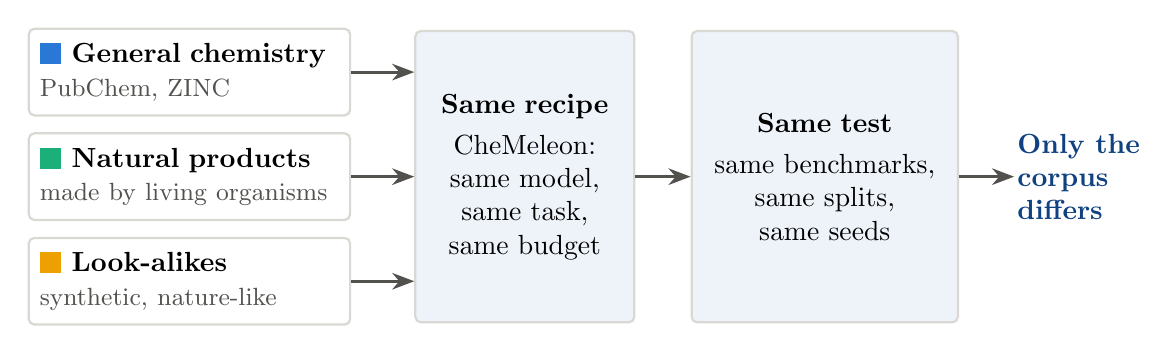
\begin{tikzpicture}[
  corp/.style={draw=hair,line width=0.8pt,rounded corners=2pt,fill=white,
    minimum height=11mm,text width=38mm,align=left,inner sep=4pt},
  fixed/.style={draw=hair,line width=0.8pt,rounded corners=2pt,fill=tint,
    minimum height=37mm,text width=25mm,align=center,inner sep=4pt},
  arr/.style={-{Stealth[length=2.8mm]},line width=1.1pt,color=ink2}]
\node[corp] (c2) {\sw{cCoco}\textbf{Natural products}\\\small\muted{made by living organisms}};
\node[corp,above=2mm of c2] (c1) {\sw{cPub}\textbf{General chemistry}\\\small\muted{PubChem, ZINC}};
\node[corp,below=2mm of c2] (c3) {\sw{cZnp}\textbf{Look-alikes}\\\small\muted{synthetic, nature-like}};
\node[fixed,right=8mm of c2] (r) {\textbf{Same recipe}\\[3pt]CheMeleon:\\same model,\\same task,\\same budget};
\node[fixed,text width=31mm,right=7mm of r] (e) {\textbf{Same test}\\[3pt]same benchmarks,\\same splits,\\same seeds};
\node[right=7mm of e,align=left,inner sep=1pt] (d) {\key{Only the}\\\key{corpus}\\\key{differs}};
\draw[arr] (c1.east) -- (r.west|-c1.east);
\draw[arr] (c2.east) -- (r.west);
\draw[arr] (c3.east) -- (r.west|-c3.east);
\draw[arr] (r) -- (e);
\draw[arr] (e) -- (d);
\end{tikzpicture}

\vspace{4mm}
\raggedright
\textbf{Why natural products?} Evolution shaped them, as it shaped protein
sequences, where pretraining works.\\[4pt]
{\footnotesize\muted{CheMeleon (Burns et al.\ 2026): a graph network pretrained to
predict about 1,600 computed descriptors.}}
\note{50 s. Slow down here, this is the slide to remember. The conjecture is
Prof. Barzilay's from class: merely valid molecules may be grammatical
sentences that say nothing. Two ways a gain could arise: the corpus sits
closer to the test molecules (coverage), or nature carries regularities that
help more broadly. The look-alike corpus is there to tell them apart. A clear
null counts as a result.}
\end{frame}

% =====================================================================
\begin{frame}{All the data is public, downloaded and cleaned on our cluster}
\begin{tabular}{@{}L{38mm}r@{\hspace{7mm}}L{74mm}@{}}
\toprule
\muted{Corpus, no labels} & \muted{Molecules} & \muted{What it covers}\\
\midrule
\sw{cPub}PubChem & 944,286 & general chemistry; CheMeleon's own corpus\\
\sw{cCoco}COCONUT & 738,767 & natural products\\
\sw{cZinc}ZINC sample & 499,998 & purchasable drug-like molecules\\
\sw{cZnp}ZINC look-alikes & 50,000 & its tenth most like natural products\\
\bottomrule
\end{tabular}

\vspace{4mm}
\begin{tabular}{@{}L{38mm}r@{\hspace{7mm}}L{57.2mm}L{14mm}@{}}
\toprule
\muted{Benchmark, with labels} & \muted{Molecules} & \muted{Label} & \muted{Metric}\\
\midrule
BBBP & 2,039 & crosses the blood-brain barrier? & AUROC\\
ESOL & 1,128 & water solubility (a number) & RMSE\\
\bottomrule
\end{tabular}

\vspace{4mm}
{\footnotesize\muted{Scaffold split: test molecules have ring skeletons absent
from training. Five split seeds, frozen on disk.}\\
\muted{AUROC: 0.5 is chance, 1 is perfect. RMSE: typical size of the error.}}
\note{45 s. Access is confirmed, not requested: everything is on scratch,
canonicalised and deduplicated. The same cleaning rule is applied to every
corpus. Natural-product-likeness is Ertl's 2008 score: resemblance of
structure, not biological origin.}
\end{frame}

% =====================================================================
\begin{frame}{Done: the corpora are chemically distinct, so the experiment has
a real treatment}
\begin{columns}[c,onlytextwidth]
\column{0.62\textwidth}
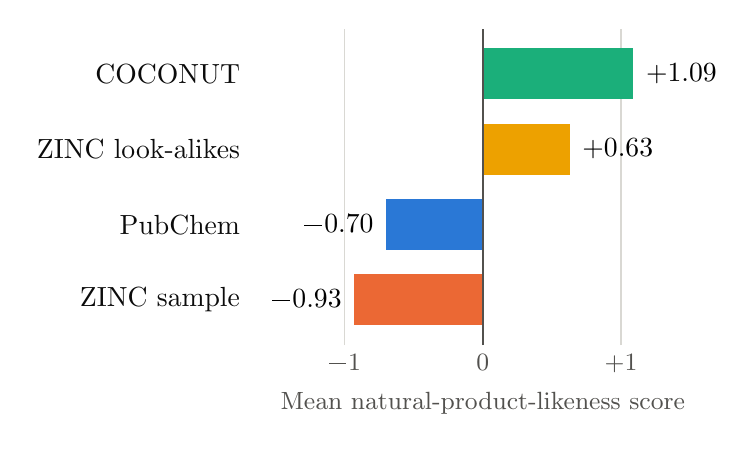
\begin{tikzpicture}
\begin{axis}[clean,
  xbar, bar width=6.5mm, bar shift=0pt,
  width=72mm, height=56mm,
  xmin=-1.6, xmax=1.6, ymin=0.4, ymax=4.6,
  ytick={1,2,3,4},
  yticklabels={ZINC sample,PubChem,ZINC look-alikes,COCONUT},
  y tick label style={font=\normalsize,color=ink},
  xtick={-1,0,1}, xticklabels={\textminus 1,0,+1},
  xmajorgrids,
  xlabel={Mean natural-product-likeness score},
  clip=false]
\addplot[fill=cZinc,draw=none] coordinates {(-0.93,1)};
\addplot[fill=cPub,draw=none] coordinates {(-0.70,2)};
\addplot[fill=cZnp,draw=none] coordinates {(0.63,3)};
\addplot[fill=cCoco,draw=none] coordinates {(1.09,4)};
\draw[ink2,line width=0.7pt] (axis cs:0,0.4) -- (axis cs:0,4.6);
\node[anchor=east] at (axis cs:-0.95,1) {\textminus 0.93};
\node[anchor=east] at (axis cs:-0.72,2) {\textminus 0.70};
\node[anchor=west] at (axis cs:0.65,3) {+0.63};
\node[anchor=west] at (axis cs:1.11,4) {+1.09};
\end{axis}
\end{tikzpicture}
\column{0.31\textwidth}\raggedright
{\fontsize{30}{34}\selectfont\bfseries\color{accent}2.15}\\[1.5mm]
standard deviations: the widest gap between two corpora on a single
property.\\[6mm]
{\footnotesize\muted{20,000 molecules per corpus. Score: Ertl et al.\ 2008,
resemblance to natural-product structures.}}
\end{columns}
\note{40 s. Before training anything we asked whether the corpora differ at
all; if not, there is nothing to measure. They do. The look-alike corpus is
only halfway to COCONUT, and we say so. The 2.15 is the share of saturated
carbons, look-alikes against PubChem. Consequence: a null result later would
mean something.}
\end{frame}

% =====================================================================
\begin{frame}{Obstacle found: PubChem already contains most benchmark
molecules, and ZINC contains none}
\begin{columns}[c,onlytextwidth]
\column{0.58\textwidth}
{\small\muted{Share of benchmark molecules found in each corpus}}\\[1mm]
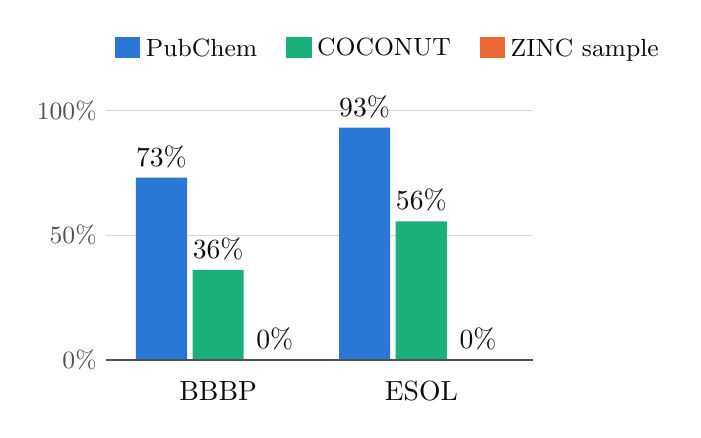
\begin{tikzpicture}
\begin{axis}[clean,
  ybar=2pt, bar width=6.5mm,
  width=70mm, height=50mm,
  ymin=0, ymax=108, xmin=0.45, xmax=2.55,
  xtick={1,2}, xticklabels={BBBP,ESOL},
  x tick label style={font=\normalsize,color=ink},
  ytick={0,50,100}, yticklabels={0\%,50\%,100\%},
  ymajorgrids,
  legend style={at={(0,1.07)},anchor=south west,legend columns=3,
    /tikz/every even column/.append style={column sep=3mm}},
  swatch legend,
  nodes near coords={\pgfmathprintnumber[precision=0]{\pgfplotspointmeta}\%},
  nodes near coords style={font=\normalsize,color=ink},
  clip=false]
\addplot[fill=cPub,draw=none] coordinates {(1,73.1) (2,93.2)};
\addplot[fill=cCoco,draw=none] coordinates {(1,36.1) (2,55.6)};
\addplot[fill=cZinc,draw=none] coordinates {(1,0) (2,0)};
\legend{PubChem,COCONUT,ZINC sample}
\draw[ink2,line width=0.7pt] (axis cs:0.45,0) -- (axis cs:2.55,0);
\end{axis}
\end{tikzpicture}
\column{0.38\textwidth}\raggedright
A win for one corpus could mean better chemistry, or test molecules already
seen.\\[4mm]
\textbf{Our plan for it}
\begin{itemize}
\setlength{\itemsep}{2mm}
\item Rerun with benchmark molecules removed from the corpus.
\item Report gains by how similar each test molecule is to the corpus.
\end{itemize}
\vspace{2mm}
{\footnotesize\muted{Exact structure matches. No label leaks: pretraining never
sees a measurement.}}
\end{columns}
\note{55 s. This is the finding we did not expect. CheMeleon's corpus is not a
uniform draw from PubChem: it holds 73 and 93 percent of our two benchmarks,
where a uniform draw would hold under one percent. In the size-matched samples
we actually train on, the overlap is one to two percent, but it is systematic
and runs in the same direction as similarity. The removal flag already exists
in our code.}
\end{frame}

% =====================================================================
\begin{frame}{Ahead of plan: 13 of 14 size-curve models are pretrained, the
last one is running}
\begin{columns}[c,onlytextwidth]
\column{0.60\textwidth}
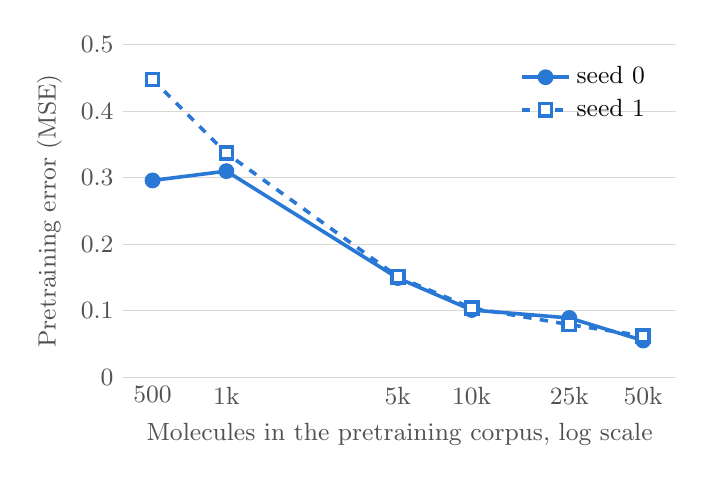
\begin{tikzpicture}
\begin{axis}[clean,
  xmode=log,
  width=86mm, height=58mm,
  xmin=380, xmax=68000, ymin=0, ymax=0.5,
  xtick={500,1000,5000,10000,25000,50000},
  xticklabels={500,1k,5k,10k,25k,50k},
  minor tick style={draw=none},
  ytick={0,0.1,0.2,0.3,0.4,0.5},
  yticklabels={0,0.1,0.2,0.3,0.4,0.5},
  ymajorgrids,
  xlabel={Molecules in the pretraining corpus, log scale},
  ylabel={Pretraining error (MSE)},
  legend pos=north east]
\addplot[cPub,line width=1.3pt,mark=*,mark size=2.2pt] coordinates
  {(500,0.296) (1000,0.310) (5000,0.149) (10000,0.101) (25000,0.089) (50000,0.055)};
\addplot[cPub,line width=1.3pt,dashed,mark=square*,mark size=2.2pt,
  mark options={solid,fill=white}] coordinates
  {(500,0.448) (1000,0.337) (5000,0.151) (10000,0.104) (25000,0.079) (50000,0.062)};
\legend{seed 0,seed 1}
\end{axis}
\end{tikzpicture}
\column{0.34\textwidth}\raggedright
The same recipe on 500 to 100,000 PubChem molecules, two seeds each: how much
data is enough?\\[5mm]
The pretraining error is still falling at 50,000.\\[5mm]
\key{Not a result yet.} The test is property prediction after fine-tuning.
\end{columns}
\note{40 s. The proposal promised one timed pilot run by today. We have the
whole size curve pretrained except one run, with checkpoint and resume tested
by a real preemption. Size comes before composition on Yuxin Xie's advice:
comparing corpora below saturation would measure size. Be plain that this
chart is a health check: the y-axis is the pretraining task and each point has
its own held-out set.}
\end{frame}

% =====================================================================
\begin{frame}{By Check-in 2: first property-prediction results}
\begin{columns}[t,onlytextwidth]
\column{0.27\textwidth}\raggedright
{\color{hair}\rule{\linewidth}{1.2mm}}\\[1.5mm]
\textbf{Done}\\[2.5mm]
Corpora audited\\[2mm]
Splits frozen, five seeds\\[2mm]
13 of 14 models pretrained
\column{0.36\textwidth}\raggedright
{\color{accent}\rule{\linewidth}{1.2mm}}\\[1.5mm]
\textbf{Check-in 2}, 17 to 24 Nov\\[2.5mm]
Fine-tuning loop, the one blocker\\[2mm]
Baselines: from scratch, plus descriptors, random forest\\[2mm]
Size curve at 50, 100, 500 and all labels
\column{0.29\textwidth}\raggedright
{\color{hair}\rule{\linewidth}{1.2mm}}\\[1.5mm]
\textbf{Final}, 1 to 10 Dec\\[2.5mm]
Corpora compared at one fixed size\\[2mm]
Benchmark molecules removed\\[2mm]
Gain against similarity to the corpus
\end{columns}

\vspace{4mm}
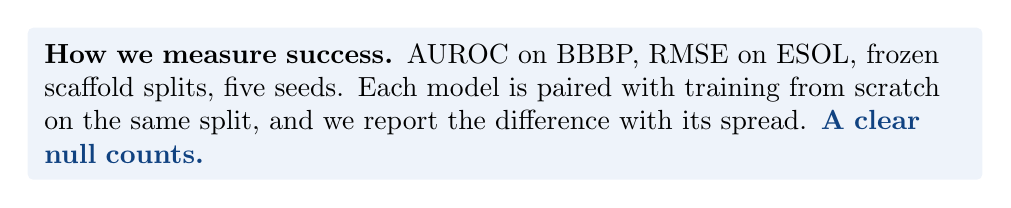
\begin{tikzpicture}
\node[fill=tint,rounded corners=2pt,inner sep=6pt,text width=\dimexpr\textwidth-12pt\relax,align=left]
{\textbf{How we measure success.} AUROC on BBBP, RMSE on ESOL, frozen scaffold
splits, five seeds. Each model is paired with training from scratch on the same
split, and we report the difference with its spread. \key{A clear null counts.}};
\end{tikzpicture}
\note{70 s. The plan in one breath: the encoders exist, the y-axis does not.
The fine-tuning protocol is already frozen, so the loop is two days of
well-specified work. The descriptor baseline matters most, because CheMeleon's
pretraining target is computed descriptors. We look hardest at 50 and 100
labels: the published gains live there. Close on the title: same model, same
training, different molecules.}
\end{frame}

% =====================================================================
% Backup slides for questions. Not part of the seven minutes.
\appendix
\renewcommand{\footlabel}{backup}

\begin{frame}{Backup: four things move together across the corpora}
\small
\begin{tabular}{@{}L{31mm}L{24mm}L{31mm}L{23mm}L{21mm}@{}}
\toprule
\muted{Corpus} & \muted{Resemblance to nature} & \muted{Property profile} &
\muted{Benchmark molecules inside} & \muted{Distance to benchmarks}\\
\midrule
\sw{cPub}PubChem & low & flat, aromatic & 73 to 93\% & nearest\\[2pt]
\sw{cCoco}COCONUT & high & large, saturated, oxygen-rich & 36 to 56\% & middle\\[2pt]
\sw{cZinc}ZINC sample & lowest & drug-like, nitrogen-rich & none & far\\[2pt]
\sw{cZnp}ZINC look-alikes & middle & small, saturated & none & farthest\\
\bottomrule
\end{tabular}

\vspace{3mm}
\normalsize\textbf{Two controls}
\begin{itemize}
\setlength{\itemsep}{2mm}
\item A PubChem sample matched to COCONUT on weight, saturation, stereocentres
and aromatic rings: does the effect survive when properties are equal?
\item One corpus with and without the benchmark molecules: does exposure drive
the effect?
\end{itemize}
\end{frame}

\begin{frame}{Backup: the effect we look for is small, and the protocol is
built for that}
\begin{tabular}{@{}L{88mm}L{46mm}@{}}
\toprule
\muted{Published benchmark, 1 October lecture} & \muted{What we do about it}\\
\midrule
Six methods not separable on ten MoleculeNet sets, Friedman p = 0.194 &
paired runs, spread reported\\[3pt]
The split alone moves AUROC from 0.78 to 0.54 & splits frozen before any run\\[3pt]
Pretraining gain on BACE: +0.07 AUROC at 60 labels, +0.04 at 847 &
low-label curves\\[3pt]
Adding descriptors to Chemprop: +0.09 AUROC at 60 labels & descriptor baseline\\
\bottomrule
\end{tabular}

\vspace{6mm}
\textbf{Fine-tuning, identical for every model.} At most 50 epochs, early
stopping with patience 10, batch 64, Adam at learning rate 0.0001, no per-model
tuning, no ensembling.
\end{frame}

\end{document}
